\documentclass[11pt,a4paper]{article}
\usepackage{amsmath,amsfonts,amssymb}
\usepackage[ngerman]{babel}
\usepackage[T1]{fontenc}
\usepackage[utf8]{inputenc}
\usepackage{longtable}
\usepackage{ae}
\usepackage{geometry}
\geometry{verbose,a4paper,tmargin=25mm,bmargin=25mm,lmargin=20mm,rmargin=20mm,nomarginpar}
\usepackage{tikz}
\usetikzlibrary{patterns}
\usepackage{graphicx}
\usepackage{mathrsfs}
\usepackage{array}
\usepackage{paralist}
\usepackage[pdfpagelabels]{hyperref}
\usepackage{pdfpages}
\usepackage{hyperref}
\usepackage{marvosym}
\usepackage{amssymb}
\usepackage{amsmath}
\usepackage{float}
\usepackage[locale=DE,separate-uncertainty=true]{siunitx}


\begin{document}
%\newcommand{\angstrom}{\mbox{\normalfont\AA}}
\newcommand*{\vertbar}{\rule[1ex]{0.5pt}{2.5ex}}
\newcommand*{\horzbar}{\rule[.5ex]{2.5ex}{0.5pt}}
\newcommand{\sg}{\vspace*{0.15cm}}
\newcommand{\pic}[4]{\begin{figure}[ht] \centering \includegraphics[width=#1\textwidth]{#2}\caption{#3}\label{#4}
\end{figure}}
\newcommand{\picoc}[3]{\begin{figure}[ht] \centering \includegraphics[width=#1\textwidth]{#2}\label{#3}
\end{figure}}

\pagenumbering{Alph}
\begin{titlepage}

\newcommand{\HRule}{\rule{\linewidth}{0.5mm}} % Defines a new command for the horizontal lines, change thickness here

\center % Center everything on the page

%----------------------------------------------------------------------------------------
%	HEADING SECTIONS
%----------------------------------------------------------------------------------------

\textsc{\LARGE Albert-Ludwigs-Universität Freiburg}\\[1.5cm] % Name of your university/college
\textsc{\Large Anfänger Praktikum I}\\[0.5cm] % Major heading such as course name
\textsc{\large Versuch 17}\\[0.5cm] % Minor heading such as course title

%----------------------------------------------------------------------------------------
%	TITLE SECTION
%----------------------------------------------------------------------------------------

\HRule \\[0.4cm]
{ \huge \bfseries   Physikalisches Pendel, Trägheitsmomente und Steinerscher Satz}\\[0.4cm] % Title of your document
\HRule \\[1.5cm]

%----------------------------------------------------------------------------------------
%	IMAGE
%----------------------------------------------------------------------------------------


\includegraphics[width=200pt]{logo}\\[1cm]


%----------------------------------------------------------------------------------------
%	AUTHOR SECTION
%----------------------------------------------------------------------------------------
\mbox{}
\vfill
\begin{minipage}{0.4\textwidth}
\begin{flushleft} \large
\emph{Versuchsteilnehmer:}\\
\underline{Andreas \textsc{Weber}},\\ \underline{Clemens \textsc{Lauby}} % Your name
\end{flushleft}
\end{minipage}
~
\begin{minipage}{0.4\textwidth}
\begin{flushright} \large
\emph{Tutor: } \\
Vorname \textsc{Nachname} % Supervisor's Name
\end{flushright}
\end{minipage}\\[1cm]

% If you don't want a supervisor, uncomment the two lines below and remove the section above
%\Large \emph{Author:}\\
%John \textsc{Smith}\\[3cm] % Your name

%----------------------------------------------------------------------------------------
%	DATE SECTION
%----------------------------------------------------------------------------------------

{\large \today}\\ % Date, change the \today to a set date if you want to be precise

%----------------------------------------------------------------------------------------
%	LOGO SECTION, if you want no logo leave this as is
%----------------------------------------------------------------------------------------

%
\includegraphics[width=200pt]{logo}\\[1cm] % Include a department/university logo - this will require the graphicx package

%----------------------------------------------------------------------------------------

\vfill % Fill the rest of the page with whitespace
\end{titlepage}



\newpage
\pagenumbering{Alph}
\numberwithin{equation}{section}
\tableofcontents
\newpage
\pagenumbering{arabic}
\section{Versuchsbeschreibung}
\subsection{Ziel des Versuches}
Das Ziel des Versuches ist es die Periodendauern eines physikalischen Pendels und eines Drehpendels experimentell zu bestimmen und diese Anhand von theorethischen Tatsachen zu vergleichen. Ebenfalls wird der Steinersche Satz mit Hilfe des Drehpendels verifiziert
\subsection{Physikalischer Zusammenhang}
       \subsubsection{Physikalisches Pendel}
       \paragraph{Periodendauer des Physikalischen Pendels}$\\$

Die Herleitung der Periodendauer des physikalischen Pendels erfolgt über die Lösung seiner Bewegungsgleichung. Die Bewegungsgleichung leitet sich über einen Zusammenhang des Drehmomentes her.\\

Das Drehmoment ist gegeben durch:
      \begin{align}
      	\vec{M} = \vec{r}\times\vec{F} = \frac{{d\vec{l}}}{dt} \\
      	\text{mit         }        \vec{l} = I \cdot \vec{\omega} \text{  und  }  \vec{\omega} = \dot{\vec{\varphi}} \notag\\
      	\text{ergibt sich:   }  \vec{M} = I \cdot \ddot{\vec\varphi}\notag
      	  \end{align}
Bzgl. eines Starren Körpers in Form eine Stabes mit Trägheitsmoment $I_a$, Masse $m_s$ und $d$ als Abstand zwischen Aufhängepubnkt und Schwerpunkt, ist der Betrag des Drehmoments folglich
\begin{equation}
		M =- I_a \ddot{\varphi}
\end{equation}
        Aus (1.1) ergibt sich:
\begin{align}
 		\vec{M}= \vec{F_G} \times \vec{d} \overset{\text{(Betrag)}}{\underset{\text{ }}{\rightarrow}} M = m_sgd \sin\varphi
\end{align}
Gleichsetzen von (1.2) und (1.3) ergibt
\begin{align*}
		 m_sgd \sin\varphi&= - I_a \ddot{\varphi} \\
 		\Leftrightarrow I_a \ddot{\varphi} + m_sgd \sin\varphi&= 0
\end{align*}
Für kleine Winkel $\varphi$ folgt
\begin{align*}
		I_a \ddot{\varphi} + m_sgd \varphi&= 0\\
		 \Leftrightarrow \ddot\varphi + \left(\frac{m_sgd}{I_a}\right)\varphi &= 0
\end{align*}
Diese Differentialgleichung hat die Form einer allgemeinen Schwingungsgleichung
\begin{align*}
	\ddot{x}+\omega^2 x = 0
\end{align*}
mit $\omega^2 = \left(\frac{m_sgd}{I_a}\right)$. Die Lösung dieser Differentialgleichung ist eine harmonische Schwingung.\\
Die Kreisfrequenz $\omega$ liefert uns durch folgende Zusammenhänge die Periodendauer
\begin{equation}
	T = \frac{1}{f} = 2\pi\sqrt{\frac{I_a}{m_sgd}} \hspace{2cm} \text{mit}\hspace{0.5cm}   f=\frac{\omega}{2\pi}
\end{equation}

\newpage

\paragraph{Trägheitsmoment des Physikalischen Pendels} $\\$

Bei Betrachtung des Ausdruckes zur Errechnung der Periodendauer ist das Trägheitsmoment $I_a$ des Oszillierenden Objektes noch Unbekannt. Dieser Abschnitt widmet sich also der Berechnung ebendieses Ausdruckes.\\

Allgemein lässt sich das Trägheitsmoment eines Starren Körpers mit Masse $m_s$ über den folgenden Ausdruck errechnen
\begin{align}
	I_s &= \int_{m}^{}  r^2_\perp \mathrm{d}m  \hspace{2cm}\text{mit  }  \varrho = \frac{m_s}{V} \notag\\
	\Rightarrow I_s &= \int_{V}^{} r^2_\perp \varrho \mathrm{d}V
\end{align}
Die Dichte $\varrho$ wird als homogen angenommen und da der Stab im Vergleich zur Länge sehr dünn ist, wird im folgenden nurnoch über die Länge $r$ integriert. Hierzu führt man die dann ebenfalls homogene Liniendichte $\lambda$ ein und erhält dann das entsprechende Trägheitsmoment für den Fall, dass die Rotationsachse Schwerpunkt des Stabes (Mitte) liegt
\begin{align}
	\lambda &= \frac{m_s}{l} \notag \\
	\overset{\text{(1.5)}}{\underset{\text{ }}{\Rightarrow}} I_s &= \lambda\int_{-l/2}^{l/2} r^2 \mathrm{d}r = \lambda \frac{l^3}{12}\notag \\
	\Leftrightarrow I_s &= \frac{1}{12} m_s l^2
\end{align}
Liegt die Rotationsachse nicht im Schwerpunkt des Stabes, erhält man ein anderes Trägheitsmoment. Im folgenden wird das Trägheitsmoment $I_a$ des Stabes berechnet, wenn die Rotationsachse im Schwerkunkt liegt. Hierfür wird der Satz von Steiner verwendet
\begin{align}
	I_a = I_s + m_s d^2 \notag
\end{align}
	In diesem Fall wählt man die Verschiebungsstrecke $d=\frac{l}{2}$, da sich der Schwerpunkt in der Mitte des Stabes Befindet. Daraus ergibt sich
\begin{align}
	 I_a = I_s +m_s \frac{l^2}{4}  \overset{\text{(1.6)}}{=} \frac{1}{3} m_s l^2
\end{align}
{\bf Letztendlich} ergibt sich die Periodendauer des physikalischen Pendels indem man Gleichung (1.7) in Gleichung (1.4) einsetzt
\begin{align}
	T = \sqrt{\frac{2l}{3g}}
\end{align}
       \subsubsection{Drehpendel}
       \paragraph{Periodendauer des Drehpendels}$\\$

Die Herleitung der Periodendauer des Drehpendels erfolgt, wie bei dem phyikalischen Pendel, ebenfalls über die Lösung der dazugehörigen Bewegungsgleichung. Die Masse des Drehpendels wird durch eine Spiralfeder zurückgetrieben. Die Feder mit Federkonstante $D$ erzeugt betraglich folgendes Rückstellmoment
\begin{align*}
	M = D \varphi
\end{align*}
Dieser Ausdruck kann mit Gleichung (1.2) gleichgesetzt werden und es ergibt sich
\begin{align*}
	I\ddot{\varphi}+D\varphi=0\\
	\Leftrightarrow \ddot{\varphi} + \frac{D}{I_{ges}}\varphi = 0
\end{align*}
Ähnlich wie beim physikalischen Pendel hat diese Differentialgleichung die Form einer allgemeinen Schwingungsgleichung mit
\begin{equation*}
	\omega^2 = \frac{D}{I_{ges}}
\end{equation*}
Für die Periodendauer der Drehtisches ergibt sich dann
\begin{align}
	T_{dt} = 2\pi \sqrt{\frac{I_{ges}}{D}}  \hspace{3cm} \text{mit } T_{dt}=\frac{2\pi}{\omega}
\end{align}
Die Größe $I_{Ges}$ beschreibt das gesamte Trägheitsmoment des Systems. Dieses setzt sich aus dem Trägheitsmoment des Drehtisches $I_{dt}$ und der Kreisscheibe zusammen. Das Trägheitsmoment der Kreisscheibe  variiert, da ihr Schwerpunkt verschoben werden kann. Dementsprechend verwendet man den Satz von Steiner. Die Zusammensetzung lautet wie folgt
\begin{align*}
	I_{ges}= I_{dt}+ I_{ks}+d^2m_{ks}
\end{align*}
$m_{ks}$  ist die Masse der Kreisscheibe und $d$ ist der Abstand von dem Schwerpunkt der Kreisscheibe zur Rotationsachse. $I_{ges}$ eingesetzt in (1.9)  und umgeformt ergibt dann
\begin{align}
	T_{dt} = 2\pi\sqrt{\frac{I_{dt}+ I_{ks}+d^2m_{ks}}{D}}\notag\\
	\Leftrightarrow {T_{dt}}^2 = 4 \pi^2 \left(\frac{I_{dt}+ I_{ks}+d^2m_{ks}}{D}\right)
\end{align}
\paragraph{Trägheitsmoment der Kreisscheibe}$\\$

Die Masseverteilung der Kreisscheibe mit wird als homogen angenommen. Der allgemeine Ausdruck lautet wie folgt
\begin{align*}
	I_{ks} = \varrho\int_{V}^{}r^2\perp\mathrm{d}V
\end{align*}
Die Kreisscheibe hat die Form eines Zylinders mit Volumen $V $, Höhe $h$ und Radius $R$ .Für die berechnung bieten sich Zylinderkoordinaten an mit $\mathrm{d}V=r\hspace{0.15cm}\mathrm{d}r\mathrm{d}\varphi\mathrm{d}y$.
Für das Integral ergibt sich dann
\begin{align*}
	I_{ks} &= \frac{m_{ks}}{V} \int_{0}^{h}\int_{0}^{2\pi}\int_{0}^{R} r^3 \mathrm{d}r\mathrm{d}\varphi\mathrm{d}y \\
	\Leftrightarrow I_{ks} &= \frac{1}{2} m_{ks}R^2
\end{align*}
Wenn $I_{ks}$ in (1.10) eingesetzt wird, ergibt sich dann letztendlich
\begin{align*}
	{T_{dt}}^2 &= 4 \pi^2 \left(\frac{I_{dt}+ \frac{1}{2} m_{ks}R^2}{D}\right) +4\pi^2 \left(\frac{d^2m_{ks}}{D}\right)\\
	\text{Def: } a&:= 4\pi^2\left(\frac{I_{dt}+\frac{1}{2}m_{ks}R}{D}\right) \text{;  } \hspace{2cm}b:= 4\pi^2\frac{m}{D}\\
	\Rightarrow I_{dt} &= \frac{Da}{4\pi^2}-\frac{1}{2}mR^2\text{ ; }\hspace{2.6cm}\Rightarrow D = \frac{4\pi^2 m_{ks}}{b}
\end{align*}
Es liegt nun also der linearer Zusammenhang $T^2=a+bd^2$ vor. Durch lineare Regression kann man $a$ und $b$ bestimmen und folglich das Trägheitsmoment des Drehtisches und die Federkonstante der Spiralfeder bestimmen.





\subsection{Versuch zum Aufgabenteil 3}
      \subsubsection{Versuchsaufbau}
      \begin{figure}[h]
      	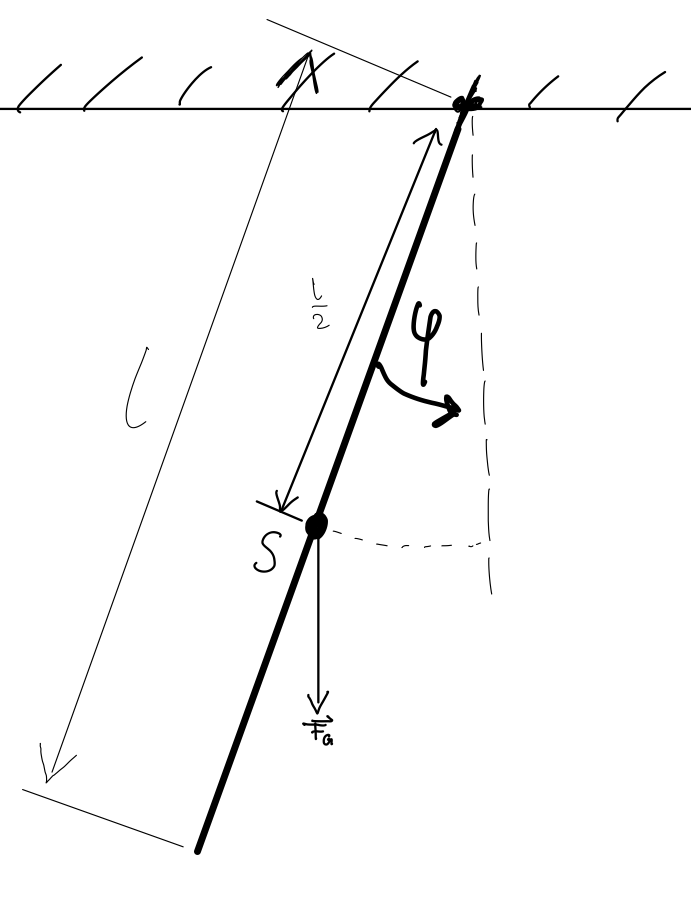
\includegraphics[width=0.4\linewidth]{physikalisches Pendel.png}
      	\centering
      	\caption{Darstellung eines physikalischen Pendels \text{[1]}}
      \end{figure}
Das in Abbildung 1 gezeigte Pendel  ist ein Zylinderförmiger Metallstab, der in einer Ebene Oszillieren kann. Die Dichte wird als homogen angenommen. Folglich beschreibt $\varphi$  den Auslenkwinkel des Pendels, $l$ die Gesamtlänge und S symbolisiert den Schwerpunkt. Der Abstand $d$ zwischen Aufhängepunkt und Schwerpunkt entspricht $\frac{l}{2}$.
      \subsubsection{Durchführung}

Ziel des ersten Versuches ist es die Periodendauer des Pendels Anhand zwei unterschiedlicher Messmethoden zu bestimmen. Um diesen Versuch durchzuführen bestand die erste Methode daraus, 30 Einzelmessungen durchzuführen und die Zeit für eine einzelne Schwingung zeitlich mit einer Stoppuhr zu messen. Dazu wurde das Pendel ca. um $10^\circ$ ausgelekt.
 Die Zeitmessung erfolgte zwischen dem ersten und einem weiteren durchlaufen des Umkehrpunktes.
 Die Zweite Methode bestand daraus, eine zeitliche Messung von 30 Perioden mit den gleichen Versuchsbedingungen durchzuführen. 
 Da man für die theorethische Errechnung der Periodendauer die Länge des Pendels braucht, wurde die Länge des Matallstabes von Aufhängepunkt bis Stabende mit einem Maßband gemessen.

\subsection{Versuch zum Aufgabenteil 4}

     \subsubsection{Versuchsaufbau}
     \begin{figure}[H]
     	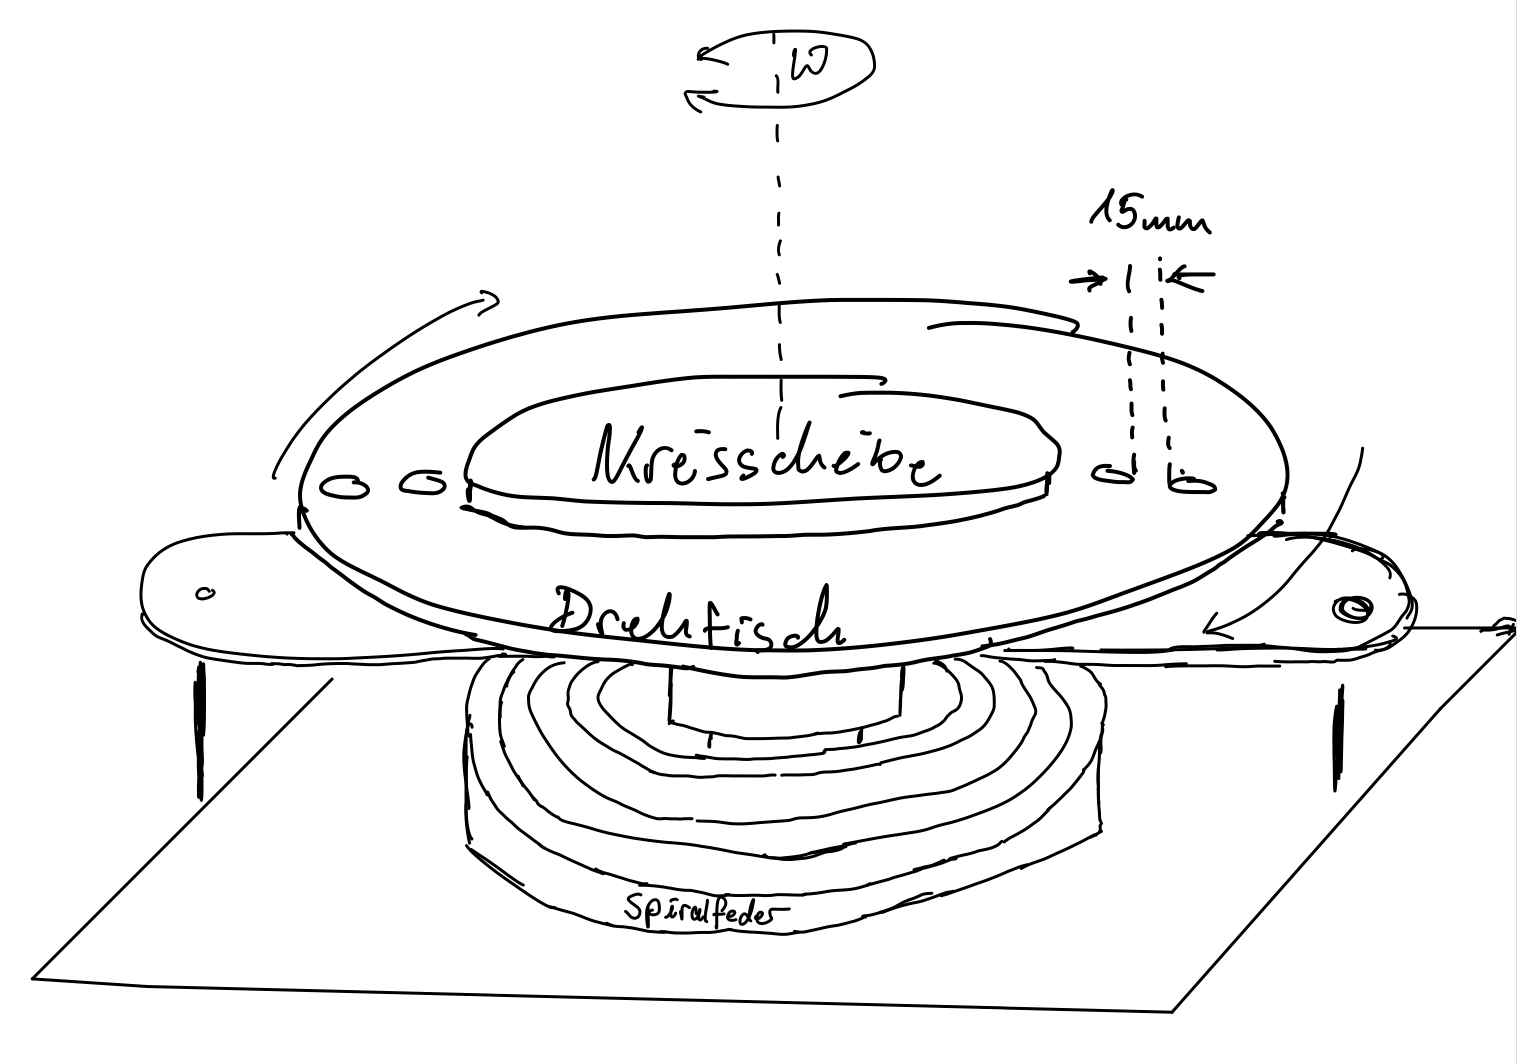
\includegraphics[width=0.6\linewidth]{Drehpendel.png}
     	\centering
     	\caption{Darstellung eines Kreispendels \text{[2]}}
     \end{figure}
 Der in Abbildung 2 gezeigte Versuchsaufbau besteht aus einem Stativ, das von einer Welle Durchführt wird. Auf dem oberen Teil der Welle Sitzt ein Drehteller, sodass das Schwerpunkt des Drehtellers auf der Rotationsachse der Welle liegt. In den unteren Teil der Welle ist eine Feder eingehängt, sodass der Drehteller durch Rotation in Schwingung versetzt werden kann. Auf dem Drehteller befinden sich 7 Löcher mit jeweils 15mm Abstand, die von der Mitte nach Außen hin angeordnet sind.
     \subsubsection{Durchführung}
Ziel des Versuches ist es, die Periodern für unterschiedliche Gewichtsverteilungen zu Messen. Dazu wurden 8 Einzelmessungen von jewiels 10 Schwingungsperioden zeitlich gemessen.
Die erste Messung erfolgte ohne Kreisscheibe. Bei der zweiten Messung wurde die Kreisscheibe mit dem Schwerpunkt auf die Drehachse des Drehtiischs gelegt. Bei den 6 weiteren Messungen wurde der Schwerpunkt der Kreischeibe jeweils um 15mm Abstand zur Drehachse verschoben.
Da zur Berechnung des Trägheitsmomentes der Kreisscheibe der Radius bzw. der Durchmesser benötigt wird, wurde dieser mit einem Messschieber gemessen.
\section{Auswertung und Fehleranalyse}
	\subsection{Physikalisches Pendel}

	Im ersten Teil unseres Versuches haben wir 30 mal die Periodendauer einer Schwingung des Pendels
	gemessen. Aus den 30 Messwerten errechnen wir den Mittelwert mit:

	\begin{equation}
	\bar{T} = \frac{1}{n} \sum_{i=1}^{n} T_i
	\end{equation}
	Die Standardabweichung mit:
	\begin{equation}
	s_T=\sqrt{\frac{1}{n-1}\sum_{i=1}{n} (T_i - \bar{T_s})^2}
	\end{equation}
	Die Standardabweichung des Mittelwerts mit:
	\begin{equation}
	s_{\bar{T}}=\frac{s_T}{\sqrt{n}}
	\end{equation}
	Das Ergebnis bezüglich unserer 30 Messwerte (siehe Anhang) ist also:
	\begin{equation*}
	\bar{T_e}=(1.5850 \pm 0.0081)s
	\end{equation*}
	\\
	Im zweiten Teil des Versuches haben wir die Schwingzeit von 30 Perioden gemessen. \\
	Dabei haben wir unsere Messungenauigkeit auf $\pm 0.1$s abgeschätzt. Also ist $T_{30}=(48.03\pm 0.1)s$
	\\
	Die Schwingungsdauer einer Periode berechnet sich als:
	\begin{equation*}
	\bar{T}=\frac{T_{30}}{30}
	\end{equation*}
	Mit einer Standardabweichung von $$\frac{s_{T_{30}}}{30}=\frac{0.1}{30}[s]\approx 0.003[s]$$
	Also ist $\bar{T_r}=(1.601\pm 0.003)s$. \\
	Um die Verträglichkeit der beiden Periodendauern zu bestimmen verwenden wir:
	\begin{equation}
	t=\frac{ |x_0 -y_0|}{\sqrt{(\Delta x)^2 + (\Delta y)^2}}
	\end{equation}
	Für unsere Werte und Unsicherheiten ergibt sich $t=1.96<2$. Also sind unsere Ergebnisse verträglich.
	\newpage
	Vergleicht man das Ergebnis der 30 Einzelmessungen mit dem der Messung von 30 Schwingungen,
	so fällt auf, dass die Standardabweichung bei der Messung von einer einzelnen Periode deutlich
	größer ist als die Standardabweichung einer Periode bei der Messung von 30 Schwingungen.
	Bezüglich diesem Aspekt ist die Messung mehrerer Perioden der Messung einer einzelnen Periode überlegen.
	\\
	Das Ergebnis des durchgeführten T-Tests ($t=1.96$) ist zwar noch innerhalb der Akzeptanz, aber
	ziemlich nah an dem kritischen Wert von 2.
	Möglicher Grund dafür könnte eine zu niedrige Einschätzung unsere statistischer Messungenauigkeit bei der Messung von 30 Schwingungen sein.
	\\Das mehrfache durchführen der Messung von 30 Perioden hätte den Vorteil, dass man die Messungenauigkeit berechnen könnte und sich nicht auf eine Abschätzung verlassen müsste.
	\\
	Aus diesem Grund wäre eine Mischung der beiden, von uns durchgeführten, Messmethoden ideal um ein
	besonders genaues Ergebnis zu erhalten.

	\subsubsection{Bestimmung der Periodendauer}
	Aus der physikalischen Herleitung wissen wir, das T mit:
	\begin{equation}
	T=2\pi \sqrt{\frac{2l}{3g}}
	\end{equation}
	berechnet werden kann.\\
	Mit $l=(0.954\pm 0.001)$ (siehe Protokollheft) \\ und $g=9.81$(Demtröder: Experimentalphysik 1,Springer,2018,s.25)
	sowie der Gaußschen Fehlerfortpflanzung:
	\begin{equation}
	\Delta z = \sqrt{(\frac{\partial f}{\partial x}\Delta x)^2 +(\frac {\partial f}{\partial y} \Delta y)^2+...} \text{   für   } z=f(x,y,...)
	\end{equation}
	ergibt sich T rechnerisch zu: $T_{rech}=(1.599830\pm0.000054)$s\\
	{\bf Diskussion der Abweichung zwischen berechneter und gemessener Schwingungszeit}\\
	Ein T-Test (2.4) zwischen den Werten $T_e$ und $T_{rech}$ ergibt $t=1.82<2$(wobei $\Delta T_{rech}$ im Vergleich zu $\Delta T_e$ sehr klein ist und deswegen in der Berechnung von t vernachlässigt werden kann).\\
	Also sind die Abweichungen zwischen dem berechnetem Wert und dem experimentell bestimmten Wert
	verträglich miteinander. Unser , durch Messen bestimmtes, Ergebnis stimmt also mit der theoretischen Herleitung überein.


	\subsection{Drehpendel / Versuchsteil 4}
	In diesem Versuchsteil benutzen wir ein Drehpendel um den Steinerschen Satz zu verifizieren.
	Wir führten 8 Einzelmessungen, welche je die  Dauer von je 10 Perioden, bei unterschiedlichen Versuchsaufbauten, gemessen haben.\\
	Für die Zeitmessung der Zehn Perioden schätzen wir die Messungenauigkeit, wie beim physikalischem pendel, auf $s_{10p}=\pm 0.1$[s] ein.\\
	unsere Messungenauigkeit bzgl. einer Periode beträgt also $s_p=\pm \frac{0.1}{10} =0.01$ [s]
	\\
	Uns interessiert zunächst die Periodendauer des Pendels ohne Kreisscheibe. Aus den Messwerten
	ergibt sich diese zu $$T_{DT}=(2.10\pm 0.01)s$$
	Aus Gleichung (***) wissen wir, dass für das Drehpendel ohne aufgelegtes Gewicht folgende Gleichung gilt:
	\begin{equation}
	T_{DT}=2 \pi \sqrt{\frac{I_{DT}}{D}}
	\end{equation}
	Umstellen ergibt:
	\begin{equation}
	\frac{I_{DT}}{D} = \frac{T_{DT}^2}{4 \pi^2}=0.1117[\frac{kg\cdot m}{N}]
	\end{equation}
	Mithilfe der Gaußschen Fehlerentwicklung (2.6) berechnet sich diesbezüglich der Fehler als $\pm 0.0033
	\frac{kg \cdot m}{N}$
	Also Ist $$\frac{I_{DT}}{D} =(0.1117 \pm 0.0033)\frac{kg\cdot m}{N}$$
	Als nächstes wollen wir das Trägheitsmoment der Kreisscheibe berechnen. Dazu benutzen wir:
	\begin{equation}
	I_{KS}=\frac{1}{2}m r^2 \text{  wobei  } r=\frac{1}{2} \text{Durchmesser}
	\end{equation}
	Mit unseren Werten ($m=(1158\pm 1)$g und $Durchmesser=(12.01 \pm 0.02)$cm) sowie der Gaußschen
	Fehlerentwicklung (2.6) ergibt sich:
	\begin{equation}
	I_{KS}=(2.0878 \pm 0.0072)\cdot 10^{-3} kg \cdot m^2
	\end{equation}








	Aus dem Physikalischem Zusammenhang ist bekannt, dass
	\begin{equation}
	hier formel bzgl T^2 und a^2 einfügen
	\end{equation}
	gilt.
	Auftragen von $T^2$ gegenüber $a^2$ mit den dazugehörigen Messungenauigkeiten (wobei a den Abstand der Drehscheibenrotationsachse zum Kreisscheibenmittelpunkt beschreibt) führt zu folgendem Graphen:\\
	\begin{figure}[H]
	%\includegraphics[width=500pt]{Richtkonstante}
	\caption[]{fig: $T^2$ gegen $a^2$ aufgetragen. Errorbars sehr klein, da $T^2$ nur einen Fehler von 0.002 hat}
	\end{figure}
	Die in dem Plot eingezeichnete lineare Regression $f_{reg}(a^2)=T^2=a_0 + b_0 \cdot a^2$ wurde mit:
	\begin{align}
	a_0 &= \frac{\sum x_i^2 \sum y_i -\sum x_i \sum y_i x_i}{n\sum x_i^2 -(\sum x_i)^2}=5.591[s^2]\\
	b_0 &= \frac{n \sum x_i y_i - \sum x_i \sum y_i}{n \sum x_i^2 - (\sum x_i)^2}=6.592 [\frac{s^2}{cm^2}]
	\end{align}
	Die dazugehörigen Unsicherheiten mit:
	\begin{align}
	\Delta a &= s \cdot \sqrt{\frac{\sum x_i^2}{n \sum x_i^2 - (\sum x_i^2)^2}}=0.022[s^2]\\
	\Delta b &= s \cdot \sqrt{\frac{n}{n \sum x_i^2 - (\sum x_i)^2}}=0.053[\frac{s^2}{cm^2}]\\
	 \text{wobei  } s&=\sqrt{\frac{1}{n-2} \sum [y_i -( a_0 + b_o x_i)]^2}
	\end{align}
	Um die Verträglichkeit unserer Fitparametern mit den Messwerten und deren Unsicherheiten zu bestimmen,
	verwenden wir einen Chi-Quadrat-Test:
	\begin{align}
	\chi ^2 = \frac{(\sum y_i - f_{reg}(x_i))}{s_y}
	\end{align}
	Den erhaltenen Wert teilen wir anschließend noch durch die Anzahl der Freiheitsgrade um den reduzierten Chi Wert zu bestimmen:
	$$\chi _{red} = \frac{\chi ^2 }{n-2} =3.97$$
	unser reduzierter Chi Wert liegt nicht in der Nähe von 3, ist also noch akzeptabel, dennoch ist er etwas höher als der Idealwert.
	Dies liegt wahrscheinlich daran, dass wir unseren statistischen Messfehler bei der Bestimmung der Schwingzeit zu niedrig angesetzt haben.\vspace{2cm}\\
	In dem Plot sieht man sofort, dass $T^2$ näherungsweise linear zu $a^2$ zunimmt. Diesen Zusammenhang erwarten wir aus dem Steinerschen Satz.
	\\















\subsection{Messwerte}



\newpage
\section{Anhang/Laborheft}
\begin{figure}[H]
	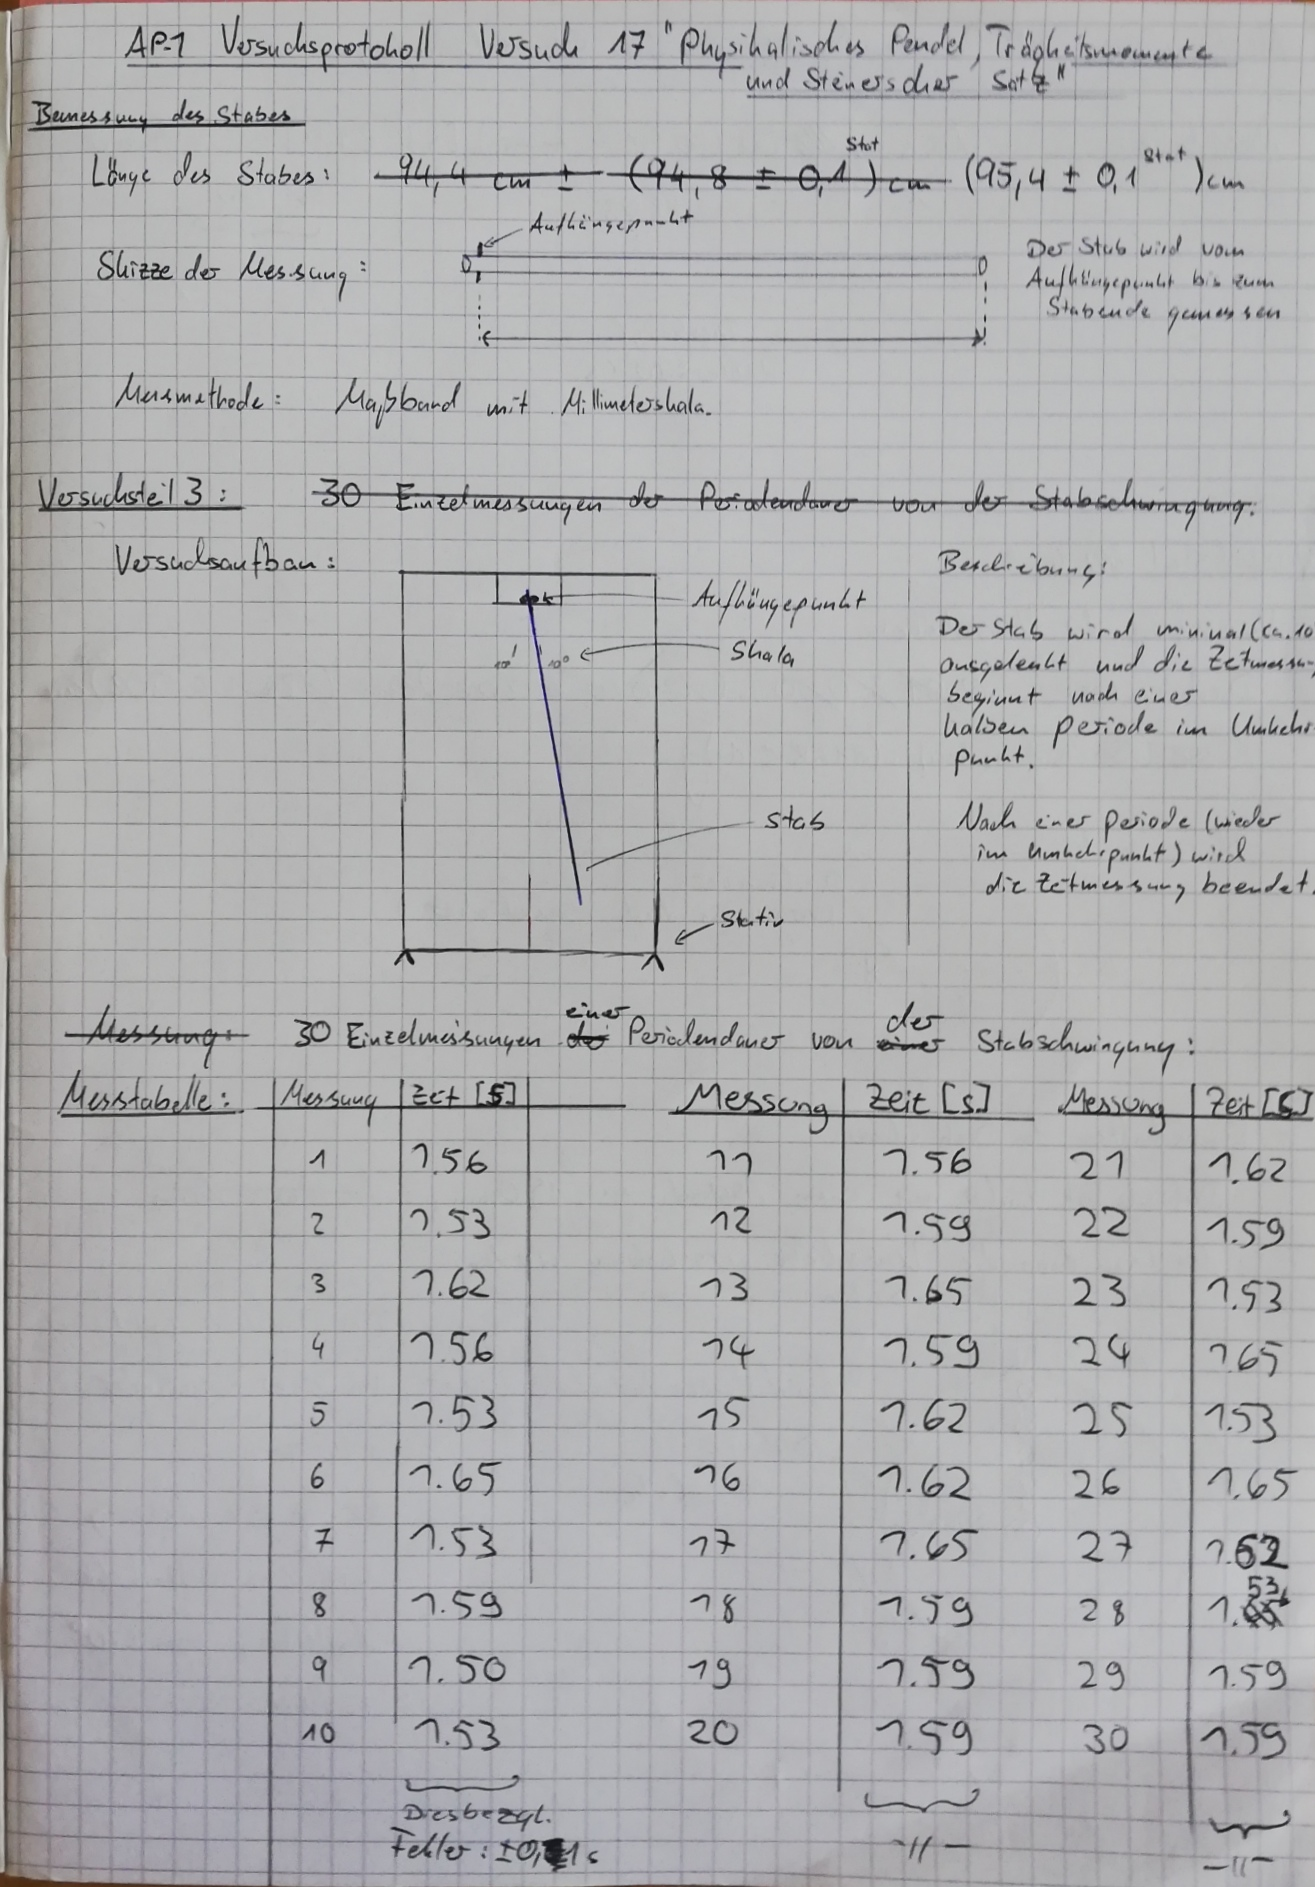
\includegraphics[width=1\linewidth]{S1.jpg}
	\centering
\end{figure}
\begin{figure}[H]
	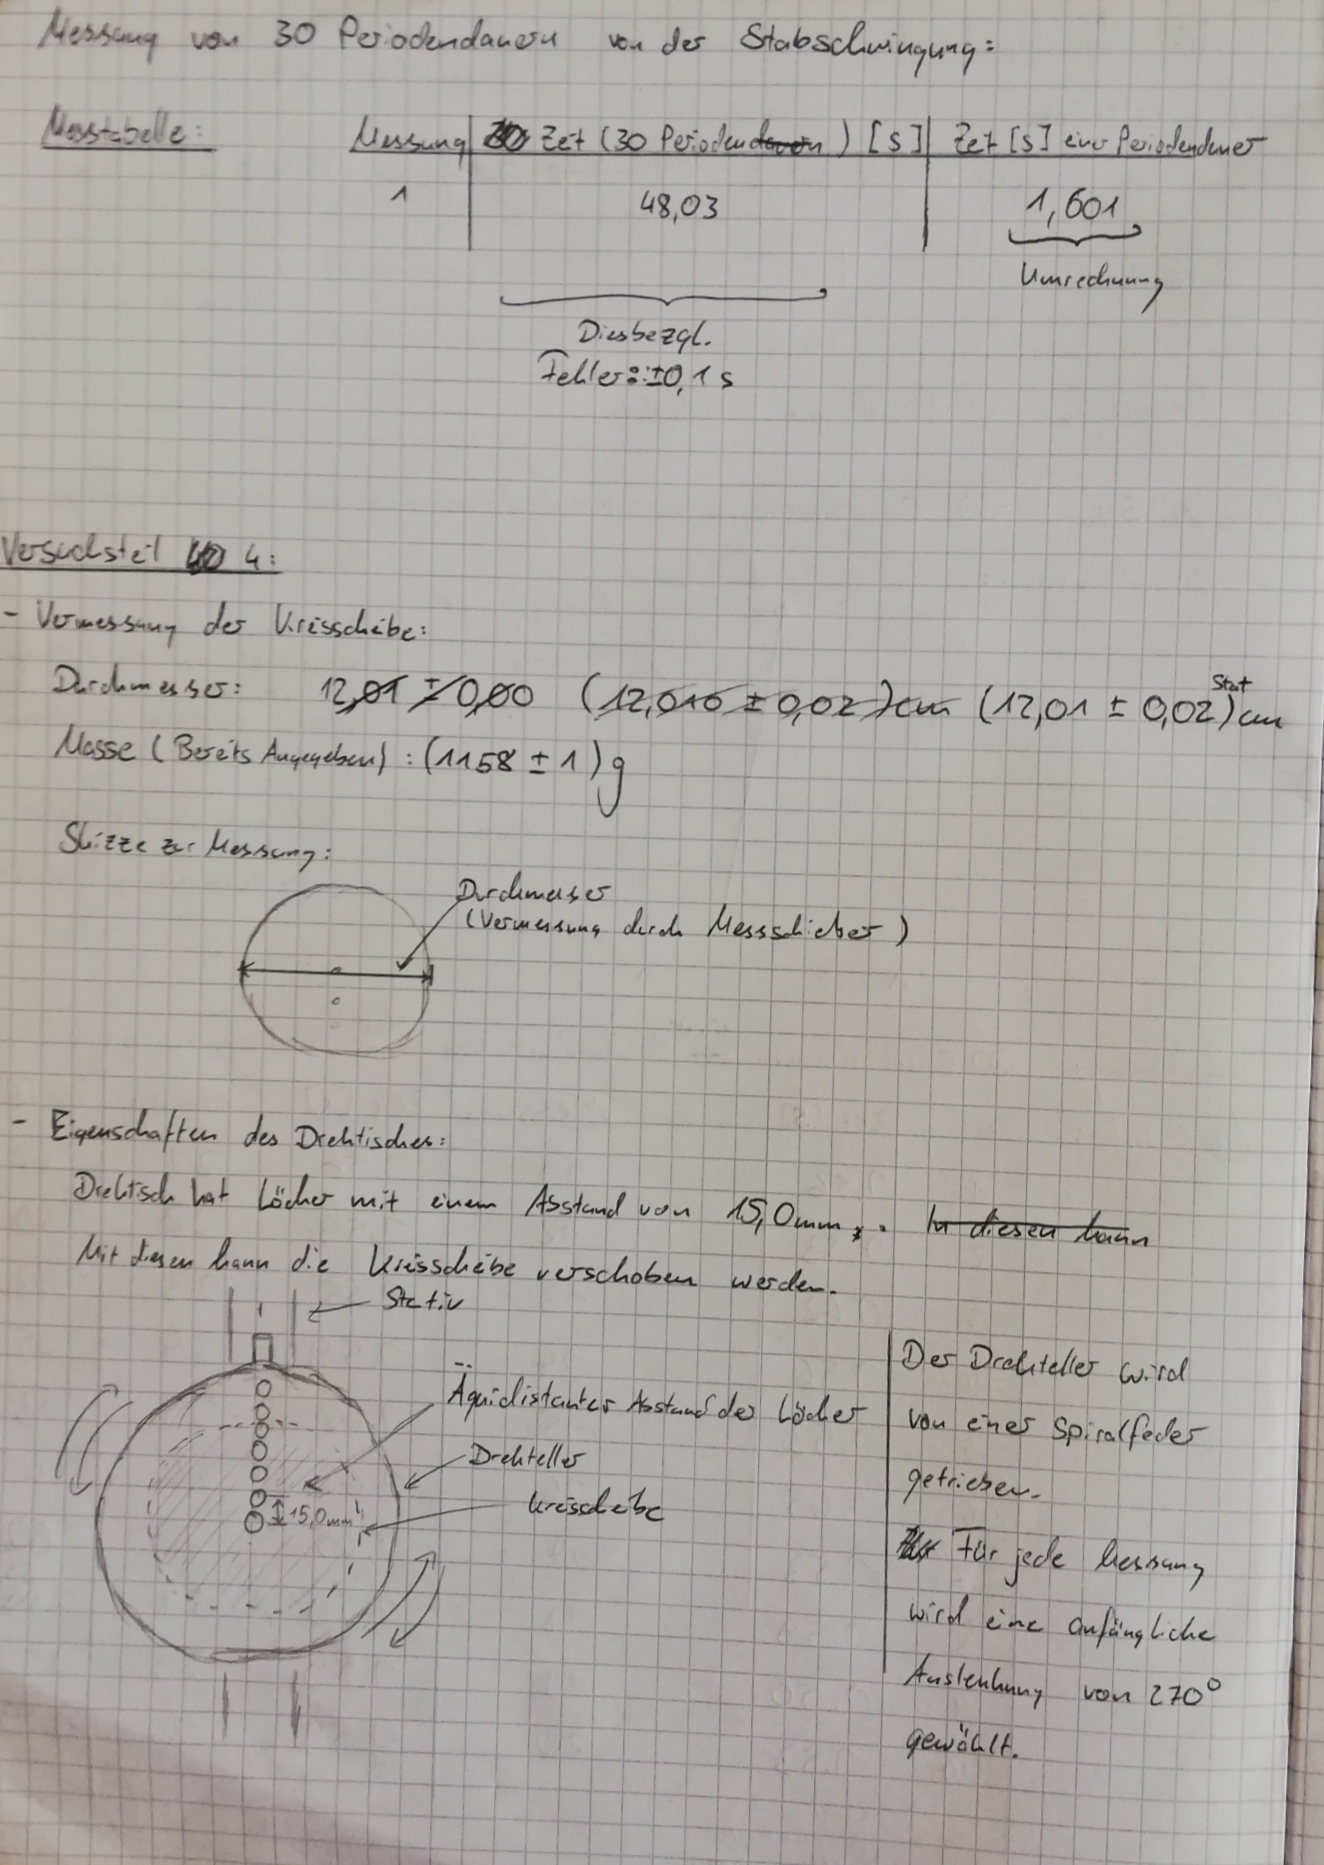
\includegraphics[width = 1\linewidth]{S2.jpg}
	\centering
\end{figure}
\begin{figure}[H]
	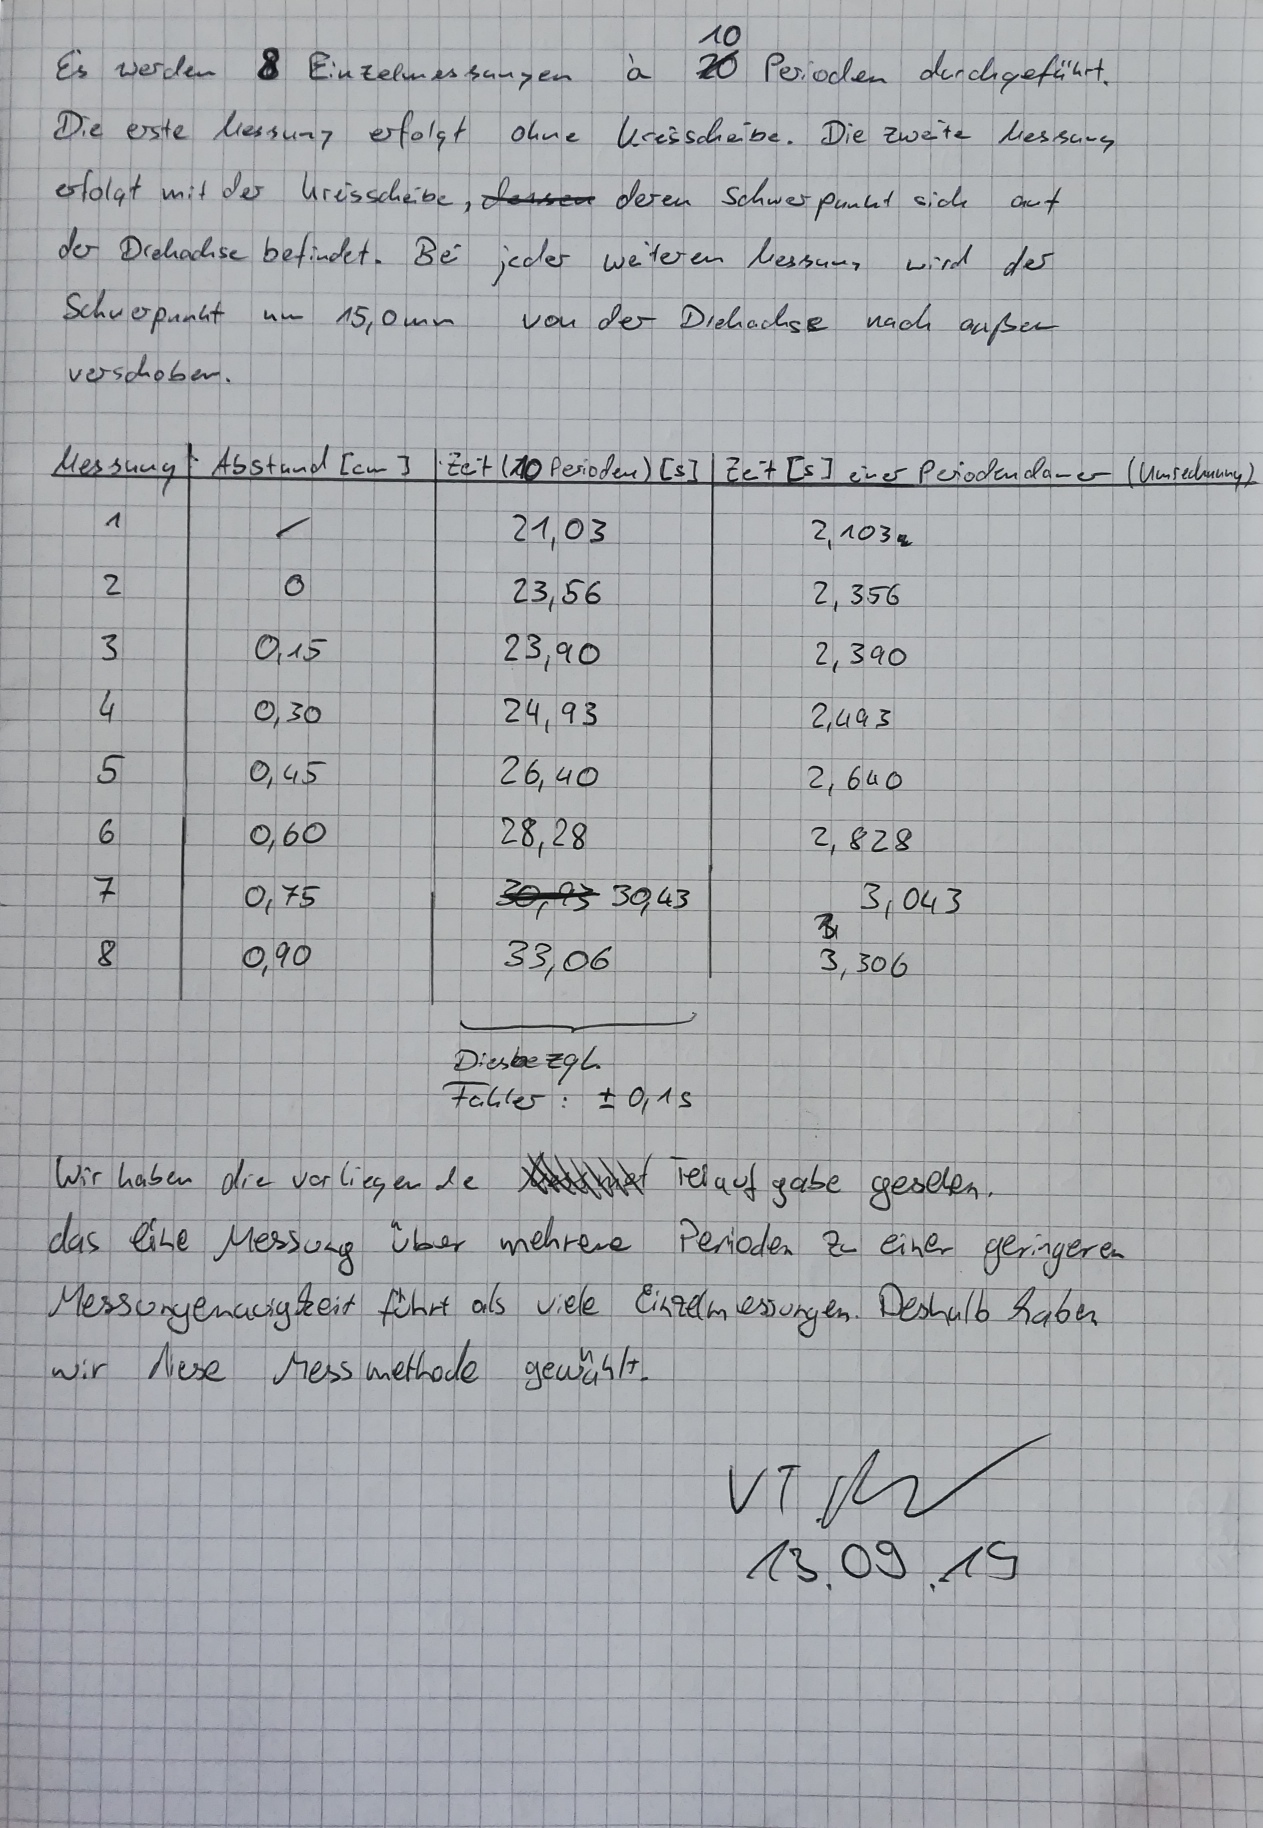
\includegraphics[width=1\linewidth]{S3.jpg}
	\centering
\end{figure}
\newpage
\section{Quellen}
\text{[1]}  \hspace{2cm} Selbsterstellte Zeichnung mit Notability\\
\text{[2]} \hspace{2cm} Selbsterstellte Zeichnung mit Notability\\
\text{[3]} \hspace{2cm} Größe für Erdbeschleunigung - 
%\SI{0,5+-0,1e5}{\meter}
%\bibliographystyle{apacite}


%\includepdf[pages={1-}]{abc.pdf}



\end{document}
